\chapter[Diseño y arquitectura]{Diseño y arquitectura del proyecto.}

En este capítulo vamos a explicar el método elegido para el diseño de las aplicaciones del proyecto y la arquitectura que hemos tenido que diseñar para la implementación del proyecto.

\section{Metodología de diseño usada.}

La metodología usada a lo largo de todo el proyecto a sido una metodología ágil de desarrollo. Estas metodologías fue elegida ya que se basa en dar varias iteraciones y en cada iteración se va añadiendo nuevas funcionalidades al proyecto. Normalmente esta metodología se usa por equipo de programadores pero en este caso solo estaba yo como programador y el director de proyecto fin de carrera como director del proyecto software. Al estar solo como programador, no hemos podido aplicar ninguna de las metodologías ágiles que ya existen, por lo que hemos tomado las características generales y otras que más nos interesaban de cada una.

Las características general es que es un desarrollo iterativo e incremental. Cada uno de los periodos en los que se divide el proceso de diseño e implementación se llama etapas, que deben de tener una duración de entre una a cuatro semanas y al final de cada una debemos tener una demo funcional del proyecto, esta idea nos gustó ya que después de cada reunión añadíamos cosas nuevas al proyecto y a su vez podíamos ver como iba evolucionando.  

\section{Arquitectura del proyecto.}

La arquitectura básica del proyecto es la que podemos ver en la figura~\ref{fig:arquitecturaBasica}.

\begin{figure}
  \centering
    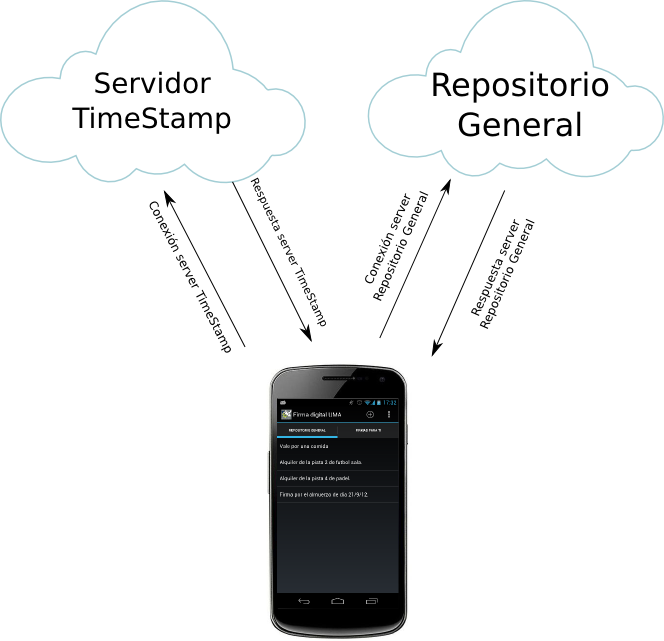
\includegraphics[scale=0.3]{./DisenhoYArquitectura/imagenes/arquitecturaBasica.png}
  \caption{Arquitectura básica del proyecto.}
  \label{fig:arquitecturaBasica}
\end{figure}

Podemos ver que la idea es tener dos aplicaciones web que son representadas por las nubes, ya que estaría en internet y una aplicación para un terminar Android. Como ya se ha explicado en capítulos anteriores las aplicaciones web se ha usado Google App Engine para el desarrollo y un terminar Android para la realización de las firmas. 

En la figura~\ref{fig:estructura} podemos ver la estructura final que tiene el proyecto, con las dos aplicaciones web diferenciadas y la aplicación del telefono.

\begin{figure}
  \centering
    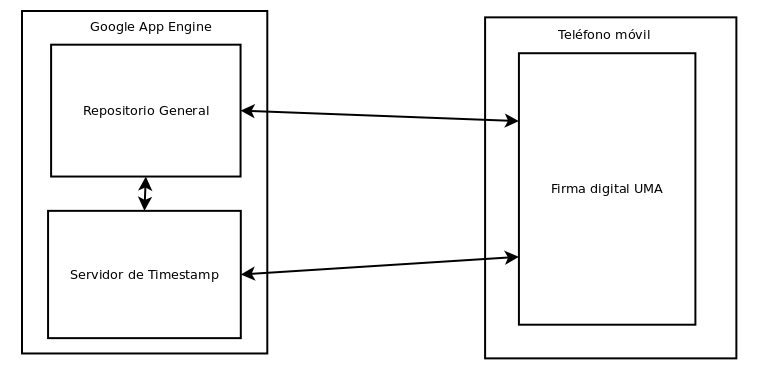
\includegraphics[scale=0.3]{./DisenhoYArquitectura/imagenes/estructura.png}
  \caption{Estructura del proyecto.}
  \label{fig:estructura}
\end{figure}

A continuación vamos a explicar cada una de las tres partes en las que se divide principalmente el proyecto.

\begin{itemize}
\item \textbf{Servidor de timestamp:} como podemos ver en la figura~\ref{fig:servertimestamp} el servidor de timestamp que hemos diseñado tiene tres partes principales, que son añadir una nueva entrada, listar una entrada determinada y listar todas las entradas para mostrarlas en la aplicación web.  
\end{itemize}

\begin{figure}
  \centering
    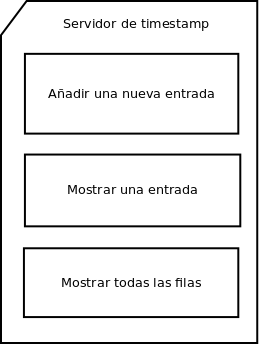
\includegraphics[scale=0.3]{./DisenhoYArquitectura/imagenes/servertimestamp.png}
  \caption{Estructura del servidor de timestamp.}
  \label{fig:servertimestamp}
\end{figure}

\begin{figure}
  \centering
    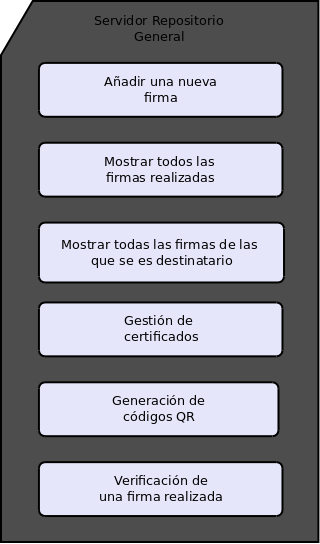
\includegraphics[scale=0.3]{./DisenhoYArquitectura/imagenes/serverRepositorioGeneral.png}
  \caption{Estructura del servidor respositorio general.}
  \label{fig:serverRepositorioGeneral}
\end{figure}

\begin{itemize}
\item \textbf{Servidor Respositorio General:} en la figura~\ref{fig:serverRepositorioGeneral} observamos la estructura básica del servidor donde tendremos el repositorio para todas las firmas realizadas y la funciones principales que nos proporciona, como pueden ser la de añadir una entrada, listar los recibos que tu has firmado o los que están dirigidos para ti, otra función importante es la gestión de certificados, la generación de código QR y la verificación de cualquier firma, para poder ver si la firma es válida o no. De todas estas funciones solo la de añadir y las de listar ambas firmas se podrán consultar con la aplicación móvil, el resto de funciones solo serán accesibles desde la aplicación web.  
\end{itemize}


\begin{figure}
  \centering
    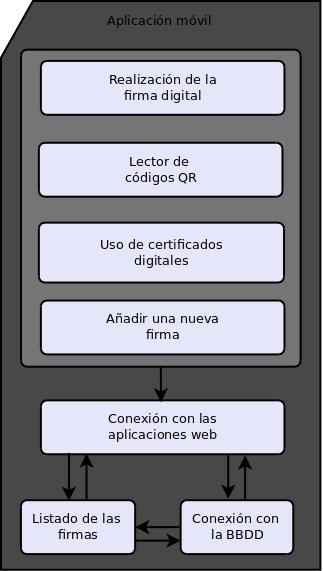
\includegraphics[scale=0.3]{./DisenhoYArquitectura/imagenes/aplicacionMovil.png}
  \caption{Estructura de la aplicación móvil.}
  \label{fig:aplicacionMovil}
\end{figure}

\begin{itemize}
\item \textbf{Aplicación Móvil:} podemos ver en la figura~\ref{fig:aplicacionMovil} la estructura general de la aplicación móvil. Como podemos ver tiene varias partes, podemos diferenciar el proceso de lectura del código QR, uso de certificados, realización de la firma digital y subirla a la aplicación web, las conexiones con las aplicaciones web, la parte de listado de las firmas y la conexión con la base de datos. Cada una de ellas tiene relación con las otras como podemos ver. El listado de las firmas podrá listarlas desde la base de datos o directamente de la aplicación web, dependiendo del caso en el que nos encontremos.
\end{itemize}










